\documentclass[11pt]{beamer}
\usetheme{Warsaw}
\usepackage[utf8]{inputenc}
%\usepackage[magyar]{babel}
\usepackage[T1]{fontenc}
\usepackage{amsmath}
\usepackage{amsfonts}
\usepackage{amssymb}
\usepackage{graphicx}
\usepackage{xurl}
\usepackage{multimedia}
\usepackage{xurl}
\newenvironment{trienv}{\only{\setbeamertemplate{items}[triangle]}}{}
\newenvironment{squareenv}{\only{\setbeamertemplate{items}[square]}}{}
\author{Bendegúz Borkovits T7UR9P}
\title{Simulating detectors with Geant4}
%\setbeamercovered{transparent} 
\setbeamertemplate{navigation symbols}{\insertframenumber/\inserttotalframenumber} 
%\logo{} 
\institute{Scientific Modeling Computer Laboratory} 
\date{March 2022} 
%\subject{} 
\begin{document}


\begin{frame}
\titlepage
\end{frame}

\begin{frame}{Geant4}
    \centering
    
\includegraphics[scale = 1.5]{g4logo.png}
    \begin{itemize}
        \vspace{0.7 cm}
        \item<tri@1-> Virtual detectors.
        \vspace{0.2 cm}
        \item<tri@1-> Support for: QT5, Python, multi-threading....
        \vspace{0.2 cm}
        \item<tri@1-> CMake project.
    \end{itemize}
    
\end{frame}


\begin{frame}{Previously...}
    \begin{itemize}
        \item<tri@1-> Setting up the environment. (VirtualBox + Ubuntu 18.04)
        \vspace{0.2 cm}
        \item<tri@1-> Installing the software. (Geant4-10.7.03)
        \vspace{0.2 cm}
        \item<tri@1-> Testing it by running an example. (B1)
        \vspace{0.2 cm}
        \item<tri@1-> Learning the stepping stones of a simulation: (via Tutorial)
        \vspace{0.1 cm}
        \begin{itemize}
            \item<square@1-> Run manager. (main function)
            \vspace{0.1 cm}
            \item<square@1-> Detector construction. (geometry, material properties)
            \vspace{0.1 cm}
            \item<square@1-> Action runner. (computation)
            \vspace{0.1 cm}
            \item<square@1-> Particle generator. (particle properties)
            \vspace{0.1 cm}
            \item<square@1-> Physics list. (laws of physics)
        \end{itemize}
        \vspace{0.2 cm}
        \item<tri@1-> Fixing issues. (optical photons, environment) FIXED!
        \vspace{0.2 cm}
        \item<tri@1-> Show output! (Compatibility issue fixed.)
    \end{itemize}
\end{frame}

\begin{frame}{Cherenkov radiation (a proton and optical photons)}
    \centering
    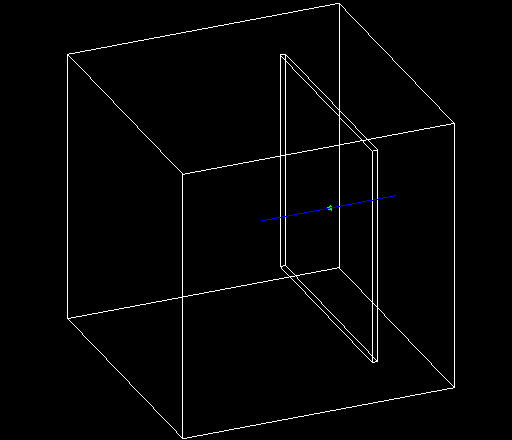
\includegraphics[scale = 0.8]{detector_volume.png}
\end{frame}

\begin{frame}{Photon cone}
    \centering
    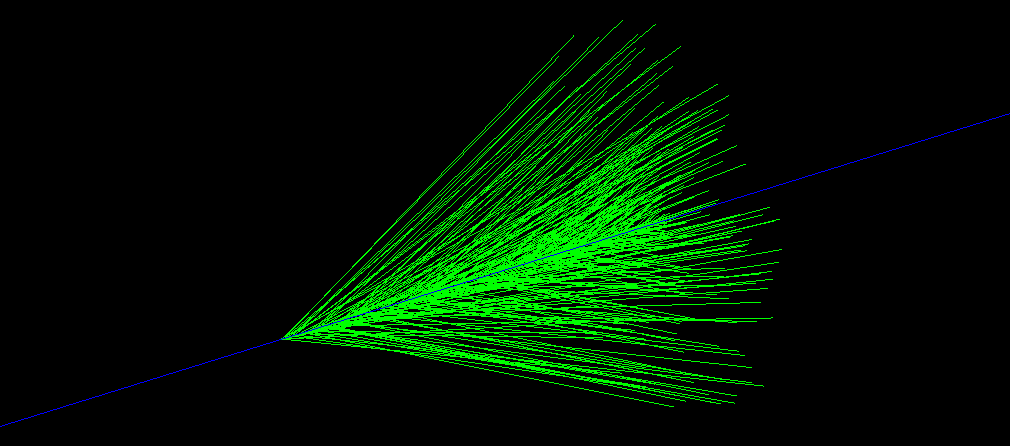
\includegraphics[scale = 0.5]{photons.png}
    \begin{itemize}
        \item<tri@1-> Electromagnetic interaction enabled in physics list.
        \item<tri@1-> A proton passes through the detector and emits photons.
        \item<tri@1-> Beta-electrons can also appear.
    \end{itemize}
\end{frame}

\begin{frame}{Continuation...}
    \centering
    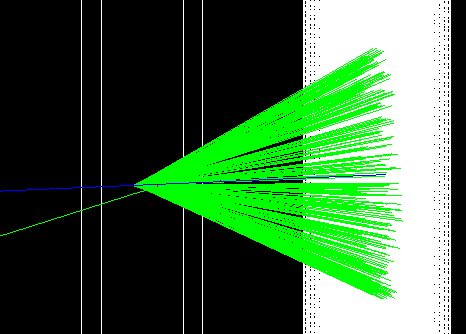
\includegraphics[scale = 0.8]{sensitive_detectors.png}
    \begin{itemize}
        \item<tri@1-> Propagating the photons through the detector.
        \vspace{0.2 cm}
        \item<tri@1-> Creating sensitive detectors.
        \vspace{0.2 cm}
        \item<tri@1-> Preparing output for analysis.
        \vspace{0.2 cm}
    \end{itemize}
\end{frame}


\begin{frame}{Saving data}
    \centering
    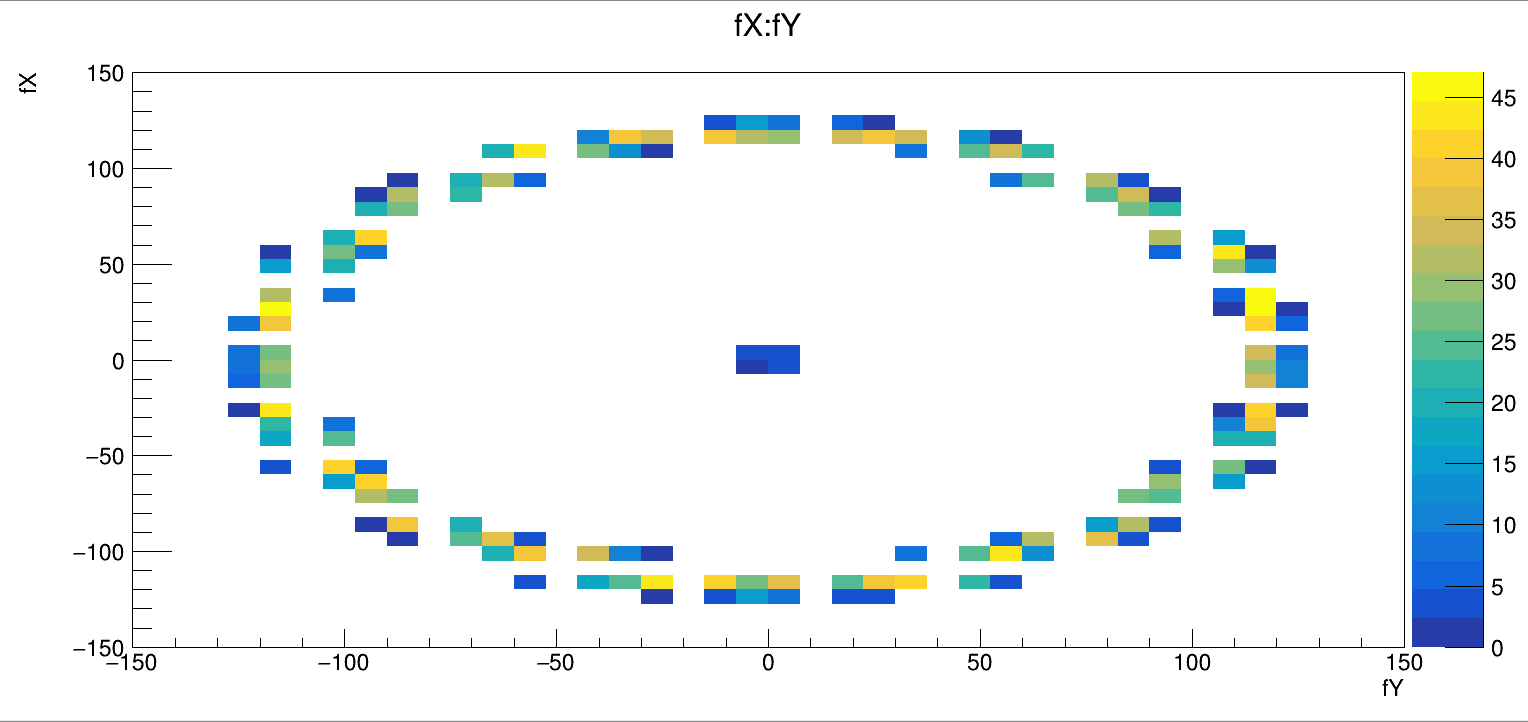
\includegraphics[scale = 0.33]{xy_phasespace.png}
    \begin{itemize}
        \item<tri@1-> Possibilities: ROOT, XML, CSV, HBOOK
        \vspace{0.2 cm}
        \item<tri@1-> Installed ROOT and checked the output. (g4root)
        \vspace{0.2 cm}
        \item<tri@1-> Opted for CSV for easier evaluation. (g4csv)
    \end{itemize}
\end{frame}

\begin{frame}{Showcasing the output}
    \centering
    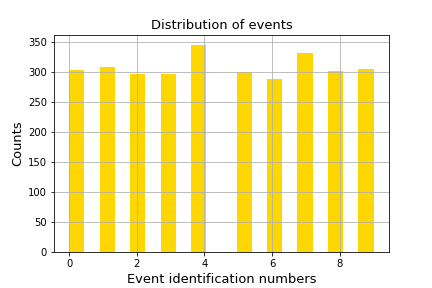
\includegraphics[scale = 0.6]{histo.png}
        \begin{itemize}
        \item<tri@1-> 10 event runs.
        \vspace{0.2 cm}
        \item<tri@1-> Counts = Number of photons in an event.
        \vspace{0.2 cm}
        \item<tri@1-> Uniformly distributed: mean of $308\pm17$ photons.
    \end{itemize}
\end{frame}

\begin{frame}{Showcasing the output}
    \centering
    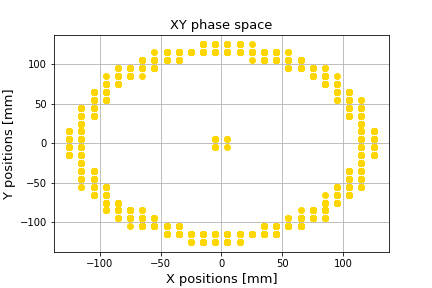
\includegraphics[scale = 0.6]{xy_phase.png}
    \begin{itemize}
        \item<tri@1-> Footprint of the photon cone.
        \vspace{0.2 cm}
        \item<tri@1-> Circular shape retrieved.
        \vspace{0.2 cm}
        \item<tri@1-> Low probability events in the middle.
    \end{itemize}
    
\end{frame}

\begin{frame}{Tools and references}
    \begin{itemize}
        \item<tri@1-> Oracle VM VirtualBox: \url{https://www.virtualbox.org/wiki/Downloads}
        \vspace{0.2 cm}
        \item<tri@1-> Ubuntu 18.04: \url{https://ubuntu.com/download/desktop}
        \vspace{0.2 cm}
        \item<tri@1-> Geant4: \url{https://geant4.web.cern.ch/support/download}
        \vspace{0.2 cm}
        \item<tri@1-> ROOT: \url{https://root.cern/install/}
        \vspace{0.2 cm}
        \item<tri@1-> Python: \url{https://www.anaconda.com/}
        \vspace{0.2 cm}
        \item<tri@1-> Tutorials: \url{https://www.youtube.com/channel/UCyxwnZPodqQR0hUo5sapRFw}
    \end{itemize}




    
\end{frame}









\end{document}
